% !TEX root = ../main.tex

\section{Results and discussion}

Here.

\subsection{Sensitivity analysis}

Results for the sensitivity analysis of the Debiagi kinetics using a batch reactor model are shown in Tables X.

\begin{figure}[H]
    \centering
    \makebox[\textwidth][c]{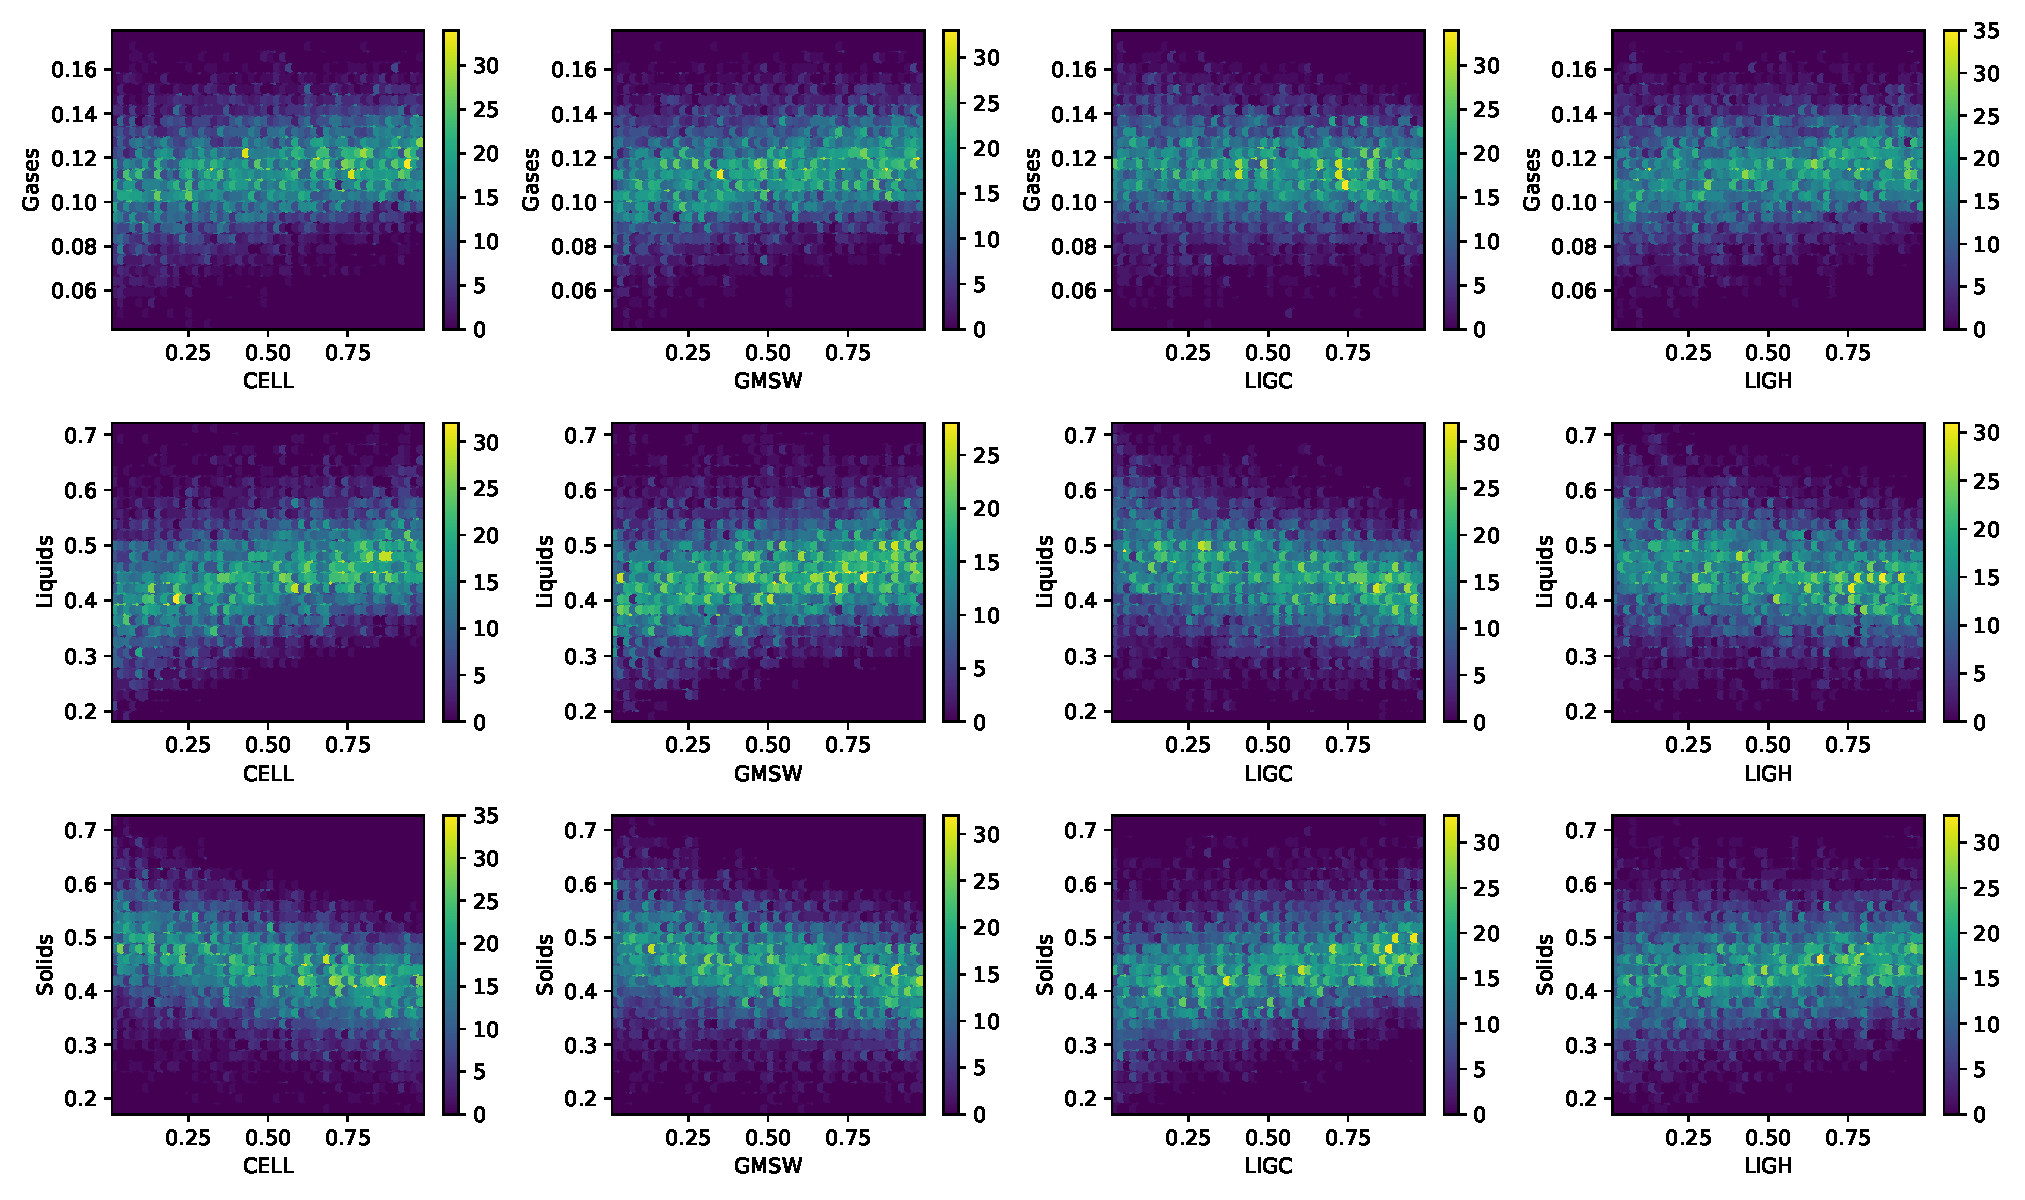
\includegraphics[width=1.3\textwidth]{figures/sa-hexbin1-n1000.pdf}}
    \caption{Batch reactor results for cellulose, hemicellulose (GMSW), carbon-rich lignin (LIGC), and hydrogen-rich lignin (LIGH) using 16,000 samples. Reaction time is 10 seconds at 773.15 K and 101,325 Pa. Colorbar represents bin count.}
\end{figure}

\begin{figure}[H]
    \centering
    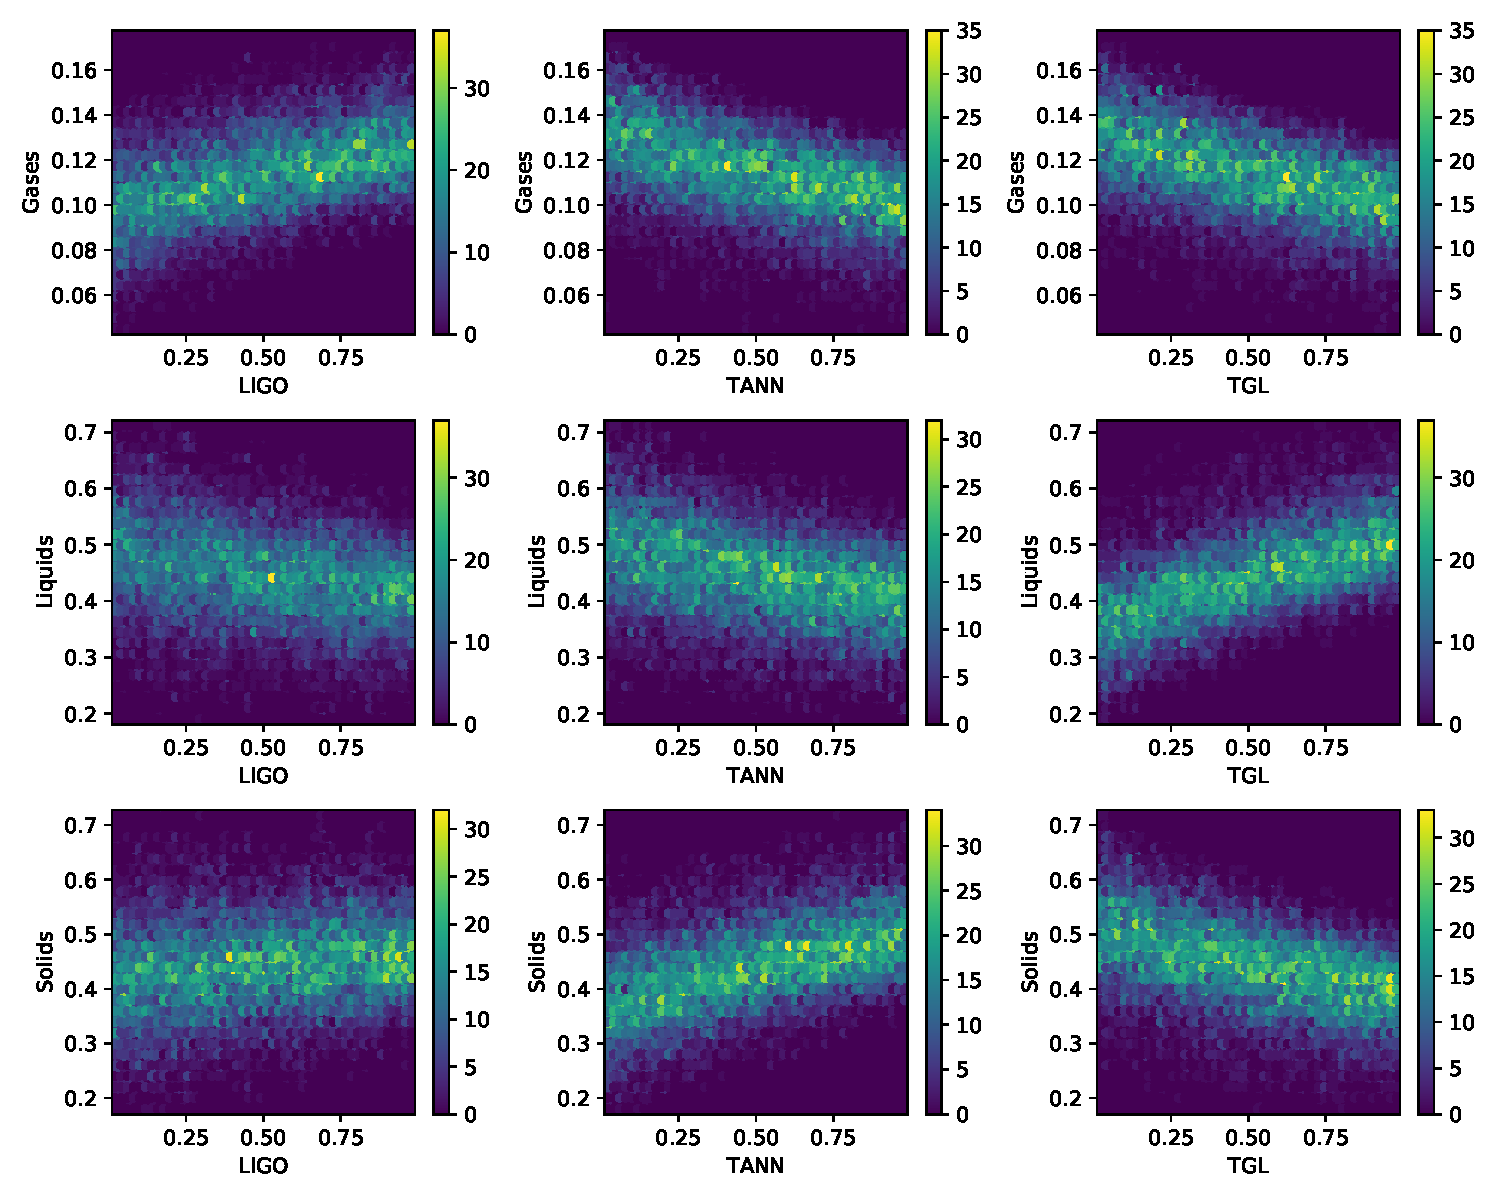
\includegraphics[width=\textwidth]{figures/sa-hexbin2-n1000.pdf}
    \caption{Batch reactor results for oxygen-rich lignin (LIGO), tannins (TANN), and triglycerides (TGL) using 16,000 samples. Reaction time is 10 seconds at 773.15 K and 101,325 Pa. Colorbar represents bin count.}
\end{figure}

\begin{figure}[H]
    \centering
    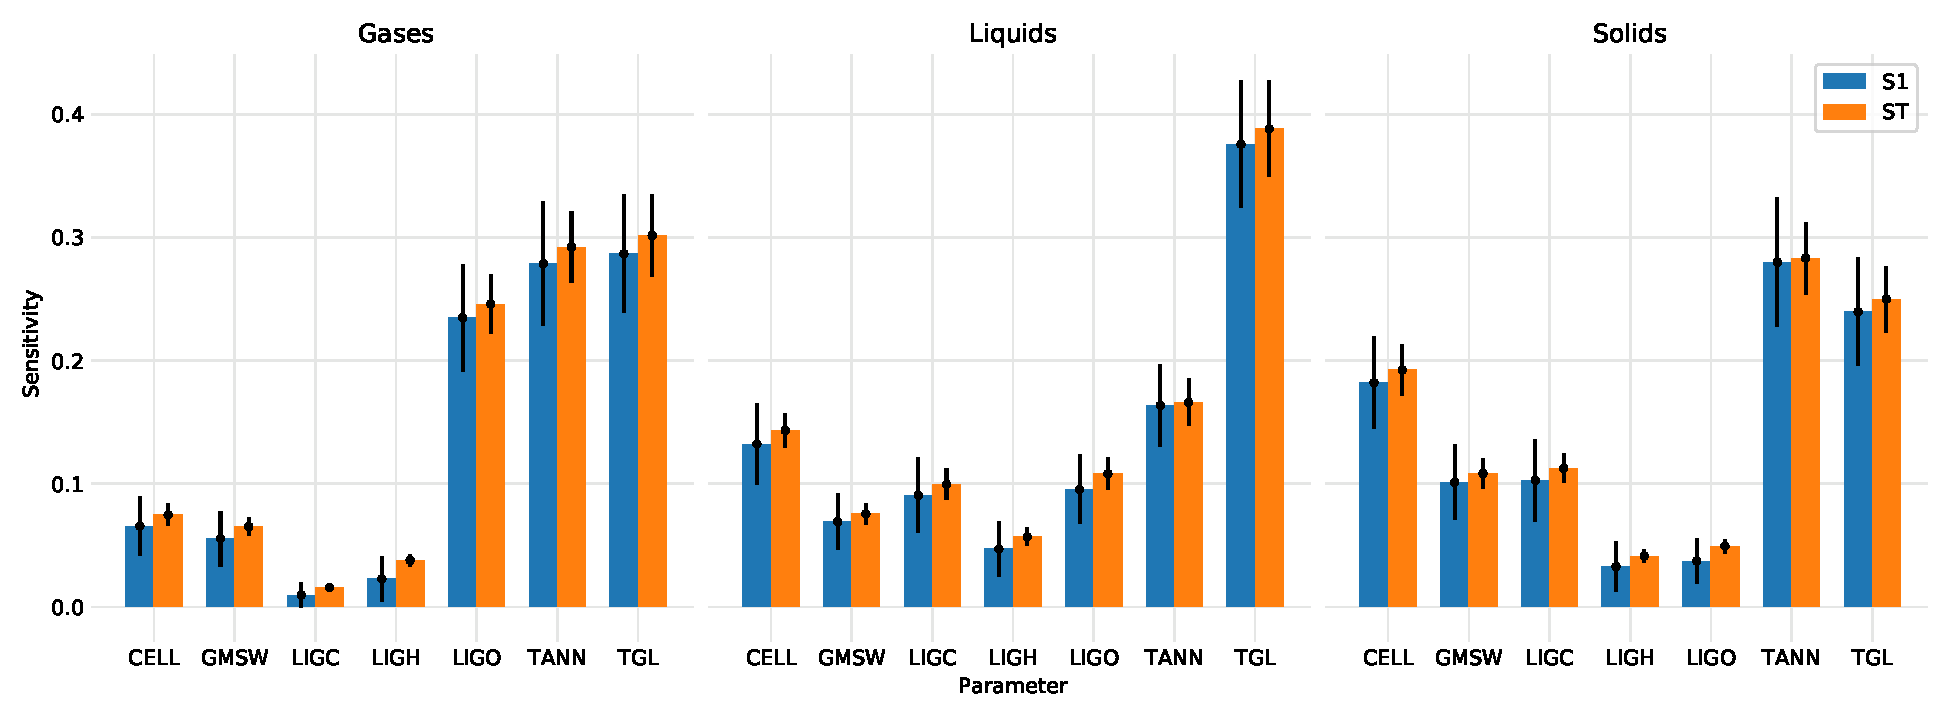
\includegraphics[width=\textwidth]{figures/sa-bar-n1000.pdf}
    \caption{First-order (S1) and total-order (ST) Sobol indices for biomass composition with reactants grouped as gases, liquids, and solids using 16,000 samples.}
\end{figure}
